\chapter{Implementacja i eksperymenty}
Nasz program został zaimplementowany w języku C z wykorzystaniem biblioteki Nauty and Traces\cite{nauty}, która umożliwia łatwe obliczeniowo wykrywanie orbit, co znacznie przyspiesza proces generowania grafów. Autorem biblioteki nauty jest Brendan D. McKay, natomiast twórcą Traces jest Adolfo Piperno. Celowo został wybrany język niskopoziomowy, ponieważ w rozwiązywaniu problemów tego typu ważna jest odpowiednia optymalizacja, co przekłada się na szybkość wykonywania programu.


Jednym z aspektów kodu, który wykorzystujemy jest sposób przechowywania grafów w pamięci komputerowej, który bazuje na macierzy sąsiedztwa. Macierz sąsiedztwa to sposób reprezentacji grafu o N wierzchołkach przy użyciu macierzy kwadratowej o wymiarach NxN. Wartość na pozycji $(m, n)$ odpowiada  krawędzi pomiędzy wierzchołkami $m$ oraz $n$ (rysunek \ref{exmatrix}).
\begin{figure}[H]
  \centering
  \hfill
  \subfloat[]{
$\begin{bmatrix}
	0 & 1 & 0 & 0 & 1 \\
	1 & 0 & 0 & 0 & 1 \\
	0 & 0 & 0 & 0 & 1 \\
	0 & 0 & 0 & 0 & 0 \\
	1 & 1 & 1 & 0 & 0 \\
  \end{bmatrix}$
  }
  \hfill
  \subfloat[]{
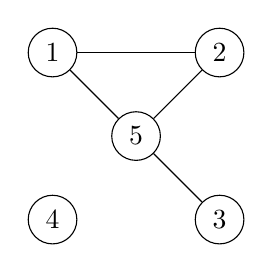
\begin{tikzpicture}[node distance={15mm}, main/.style = {draw, circle}, baseline=-8.0ex] 
    \node[main] (1) {$1$};
    \node[main] (2) [below right of=1] {$5$};
    \node[main] (3) [above right of=2] {$2$};
    \node[main] (4) [below left of=2] {$4$};
    \node[main] (5) [below right of=2] {$3$};

    \draw (1) -- (2);
    \draw (2) -- (3);

    \draw (2) -- (5);
    \draw (1) -- (3);
  \end{tikzpicture}
  }
  \hfill
  \hfill
  \caption{Graf wraz z odpowiadającą mu macierzą sąsiedztwa. W tej macierzy 0 odpowiada brakowi krawędzi, a 1 odpowiada jej istnieniu.}
  \label{exmatrix}
\end{figure}

Jako że zajmujemy się jedynie grafami prostymi i niekolorowanymi, to wartości w poszczególnych komórkach mogą wynosić jedynie 0 lub 1, oraz sama macierz jest symetryczna względem swojej diagonali. Sprawia to że macierz jest zapisywana w nadmiarowy sposób, co jednak jest niezbędne do optymalizacji obliczeń w programie. Dzięki takiemu sposobowi zapisu macierzy sąsiedztwa możemy ją traktować, nie jako tablice liczb całkowitych a jako tablice bitów. Jako że największym grafem jaki możemy uzyskać jest graf o 25 wierzchołkach to 32 bitowa wartość jest wystarczająca aby pomieścić jeden wiersz macierzy reprezentujący wierzchołek dowolnego grafu we naszym programie. Co więcej takie rozwiązanie pozwala nam bezpośrednio porównywać poszczególne wiersze macierzy jako liczby, dzięki czemu możliwe jest użycie operacji bitowych. Możliwość taka pozytywnie wpływa na optymalizacje i czas wykonania programu, przykładem jest znajdowanie sąsiadów (wykorzystane w algorytmie 1) co wykonywane jest pojedynczą operacją bitową.

Podczas implementacji algorytmu do generowania grafów Ramseyowskich o podanym stopniu (algorytm 2) sprawdziliśmy jakie znaczenie ma kolejność operacji wykluczIzomorfizmy i wykluczNieramseyowskie. Okazało się że nie ma ona znaczenia pod kątem poprawności - jednak dla grafów większych stopni operacja znajdywania orbit staje się znacznie bardziej skomplikowana w porównaniu do relatywnie prostego poszukiwania klik i zbiorów niezależnych, przez co taka kolejność poprawia ogólną efektywność algorytmu pod kątem czasu obliczeń. Aby zobrazować różnicę między dwoma algorytmami przygotowaliśmy tabelę \ref{czasgen} dla generacji grafów $R(4,4,n)$. Jak widać przy zastosowaniu optymalnego algorytmu czas generacji rośnie znacznie wolniej dla kolejnych $n$. Pomiar czasu dla $n=17$ w przypadku nieoptymalnego algorytmu został pominięty, gdyż już dla $n=12$ czas jest ten bardzo zbliżony do czasu generacji R(4,4,17) z użyciem optymalnego algorytmu.

\begin{table}[H]
 \begin{center}
 \begin{tabular}{|c c c c|} 
 \hline
 n & Liczba grafów $R(4,4,n)$ & Optymalny algorytm (sek.) & Nieoptymalny algorytm (sek.) \\ 
 \hline\hline
 1 & 1 & <1 & <1\\ 
 \hline
 2 & 2 & <1 & <1\\
 \hline
 3 & 4 & <1 & <1\\
 \hline
 4 & 9 & <1 & <1\\
 \hline
 5 & 24 & <1 & <1\\
 \hline
 6 & 84 & <1 & <1\\
 \hline
 7 & 362 & <1 & <1\\
 \hline
 8 & 2079 & <1 & <1\\
 \hline
 9 & 14701 & 4 & 4\\
 \hline
 10 & 103706 & 5 & 10\\
 \hline
 11 & 546356 & 22 & 128\\
 \hline
 12 & 1449166 & 154 & 1450\\
 \hline
 ... & ... & ... & ...\\
 \hline
  17 & 1 & 1779 & ?\\
 \hline
\end{tabular}
\end{center}
 \caption{Czas generacji grafów dla różnej kolejności wywołania wykluczIzomorfizmy i wykluczNieramseyowskie. Optymalny algorytm wywołuje te metody w kolejności wykluczIzomorfizmy i wykluczNieramseyowskie, a nieoptymalny odwrotnie}
 \label{czasgen}
 \end{table}

Jedną ze znaczących prób optymalizacji które zostały podjęte były zmiany w algorytmie tworzenia przedziałów stożków prawdopodobnych. Algorytm sklejania jest bardzo wrażliwy na ich ilość ze względu na fakt, że operacja sklejania jest wykonywana dla każdej permutacji tych przedziałów po wierzchołkach grafu $G$. Początkowo, generacja była wykonana w sposób naiwny, gdzie kolejność rozbicia przedziału była zgodna z kolejnością wierzchołków w grafie. Takie podejście produkowało jednak zbyt wiele przedziałów, i z tego powodu zostało zmienione. Kolejnym algorytmem generującym przedziały był algorytm wzorujący się na algorytmie rozszerzania przedziałów. Kolejność rozbicia była w tym przypadku zależna od kolejności wykrycia klik $K_3$. Wynik tej metody wciąż nie był zadowalający, więc podjęliśmy ponowną próbę zmniejszenia liczby przedziałów. Tym razem opierała się ona na próbach ponownego połączenia przedziałów rozbitych we wcześniejszych krokach. Takie łączenie ponownie zmniejszyło ilość przedziałów. Łączenie zostało wykonane w sposób zachłanny, i nie ma gwarancji, że daje najlepszy możliwy zbiór przedziałów. Możliwe też, że dalsze modyfikacje algorytmu tworzącego zbiór przedziałów mogłyby przynieść lepszy wynik. Średnie ilości przedziałów dla każdej z metod ich tworzenia przedstawione zostały w tabeli \ref{tabPrzedzialy}

 \begin{table}[H]
 \begin{center}
 \begin{tabular}{|c c c c|} 
 \hline
 Rząd grafów & Pierwszy algorytm & Drugi algorytm & Drugi algorytm + łączenie \\ 
 \hline\hline
 17 & 2152 &  789 & 648\\
 \hline
 16 & 1470 & 521 & 401\\
 \hline
 15 & 175 & 84 & 74\\
 \hline
\end{tabular}
\end{center}
 \caption{Tabela porównująca średnią ilość przedziałów stworzonych dla zbiorów grafów o różnych rzędach}
 \label{tabPrzedzialy}
 \end{table}
 
 Inna optymalizacja algorytmu sklejania polegała na przycinaniu drzewa permutacji przedziałów. Zasady A-D mogą spowodować ograniczenie lub odrzucenie sklejeń opisywanych przez zbiór przedziałów już na podstawie kilku pierwszych par wierzchołek-przedział. Oznacza to, że jeżeli zasady A-D będą aplikowane przed wybraniem wszystkich przedziałów, niektóre z permutacji zostaną wyeliminowanie przed wyborem wszystkich elementów, eliminując wiele możliwości jednocześnie. Na rysunku \ref{branchpruning} zostało zobrazowane odcięcie gałęzi. Dla każdego elementu drzewa wykonywane jest sprawdzenie, dzięki czemu można pominąć część rozwinięć. 
\begin{figure}[H]
\centering
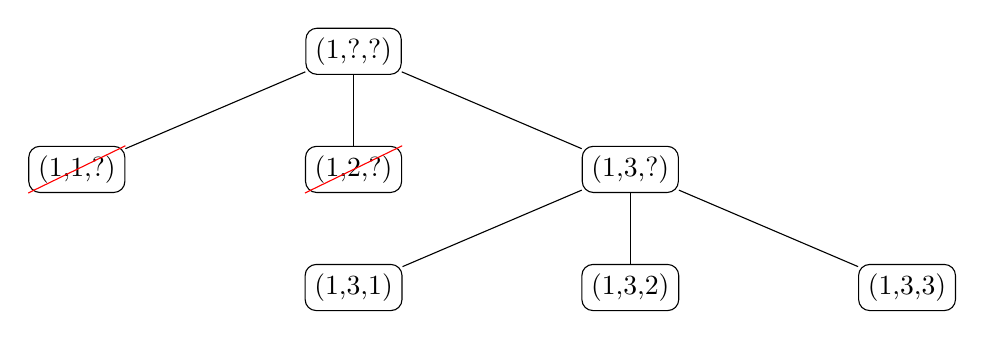
\begin{tikzpicture}[sibling distance=10em, every node/.style = {shape=rectangle, rounded corners, draw, align=center}]]
  \node {(1,?,?)}
    child { node (A){(1,1,?)}}
    child { node (B){(1,2,?)}}
    child { node {(1,3,?)}
      child { node {(1,3,1)}}
      child { node {(1,3,2)}}
      child { node {(1,3,3)} } };
   \draw[red] (A.south west) -- (A.north east);
   \draw[red] (B.south west) -- (B.north east);
\end{tikzpicture}
\caption{Zobrazowanie odcięcia gałęzi.}
\label{branchpruning}
\end{figure}
Ta optymalizacja jest absolutnie wymagana i znajdowała się już w pierwszej wersji algorytmu, ponieważ wiele permutacji może zostać odrzuconych już przy niewielkiej ilości wybranych przedziałów.